\chapter{Entwicklung des Prototpys für Visual Studio Code}
\label{cha:EntwicklungVsCode}

\section{Design}
\label{sec:EntwicklungVsCode_Design}

Um das in Kapitel \ref{cha:Prototyp} beschriebene Plugin in VS Code
zu entwickeln, werden die Komponenten verwendet, die auch in 
Abbildung \ref{fig:diagram_VSCodeDesign-Simplified} abgebildet sind.
\begin{figure}
    \centering
    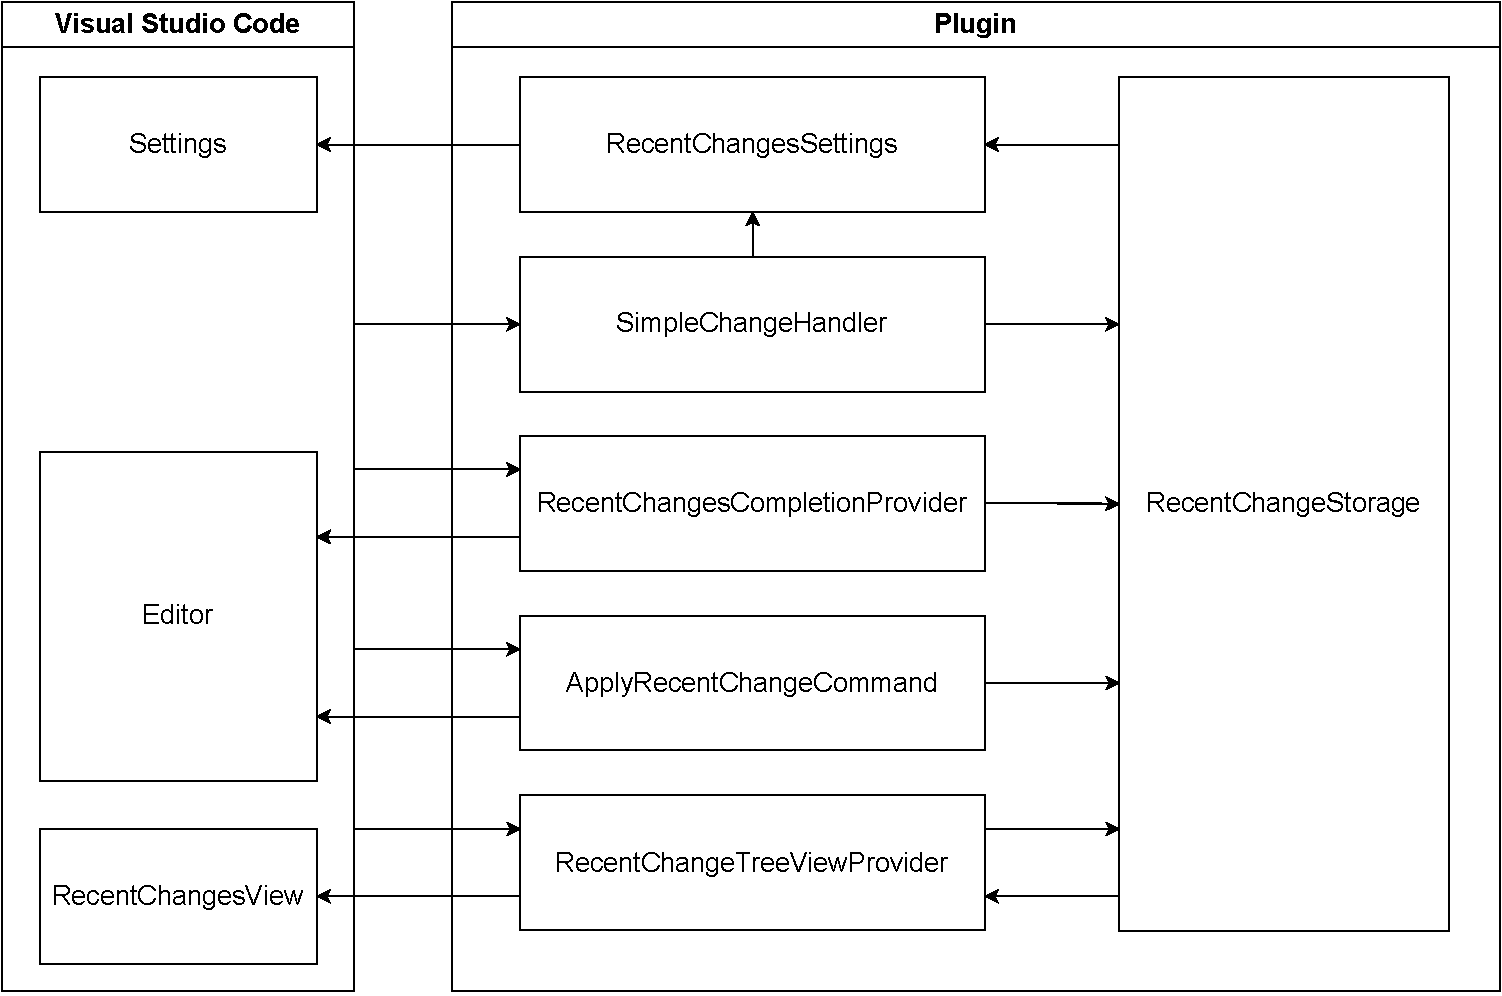
\includegraphics[width=.95\textwidth]{diagram_VSCodeDesign-Simplified}
    \caption{Stark vereinfachte Übersicht über das Design des Plugins in  VS Code.}
    \label{fig:diagram_VSCodeDesign-Simplified}
\end{figure}  

Das Herzstück des Plugins sind der \emph{SimpleChangeHandler} und
der \emph{RecentChangeStorage}. Der \emph{SimpleChangeHandler} hat die Aufgabe,
alle Veränderungen im geöffneten Dokument zu analysieren. Falls es sich um
eine verarbeitbare Veränderung handelt, wird diese im \emph{RecentChangeStorage}
gespeichert. Der \emph{RecentChangeStorage} bietet Methoden um die
gespeicherten Änderungen abzufragen und kümmert sich auch selber um das
Löschen von veralteten Änderungen.

Die Klasse \emph{RecentChangesSettings} bietet Zugriffsmethoden an,
um die von VS Code angebotenen Einstellungen abzufragen. Über sie
werden die Einstellungen für die \emph{QueueSize} (Anzahl von Veränderungen)
und die \emph{DebounceTime} (Debounce Zeit für das erkennen von Änderungen)
zugänglich gemacht.

Der \emph{RecentChangesCompletionProvider} implementiert die VS Code Schnittstelle
für Codevervollständigung. Er analysiert dabei das zu vervollständigende Wort
im Editor und fragt daraufhin den \emph{RecentChangesStorage} nach einer passenden
Änderung ab.

Der \emph{ApplyRecentChangeCommand} ist ein ausführbarer Command. Er ließt
das aktuelle Wort aus dem Editor aus, sucht im \emph{RecentChangesStorage}
nach einer passenden Änderung ersetzt und das Wort im Editor, falls
er fündig wird. Wird keine passende Änderung gefunden, so wird eine entsprechende
Nachricht angezeigt. Durch die Konfiguration des Plugins, kann der
Command auch über eine Tastenkombination aktiviert werden.

Der \emph{RecentChangesTreeViewProvider} implementiert eine Schnittstelle
um VS Code ein TreeView bereitzustellen. Die Daten für dieses TreeView
erhält er vom \emph{RecentChangesStorage}. Damit die TreeView aktuell
gehalten wird, wird der \emph{RecentChangesStorage} mithilfe eines Observer-Patterns % //TODO source
beobachtet und die TreeView bei Veränderungen aktualisiert.


% \begin{figure}
%     \centering
%     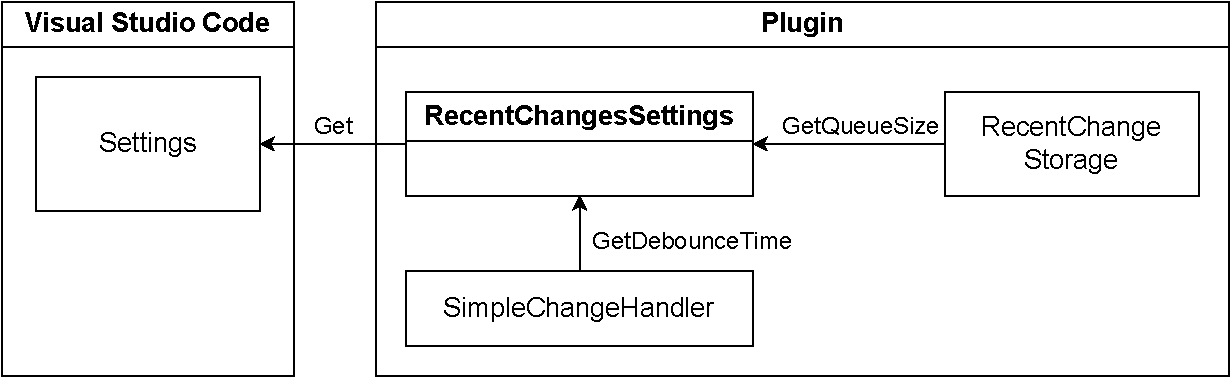
\includegraphics[width=.95\textwidth]{diagram_VSCodeDesign-Detail_Settings}
%     \caption{Detaillierte Darstellung der Komponente \emph{RecentChangesSettings}.}
%     \label{fig:diagram_VSCodeDesign-Detail_Settings}
% \end{figure} 
% \begin{figure}
%     \centering
%     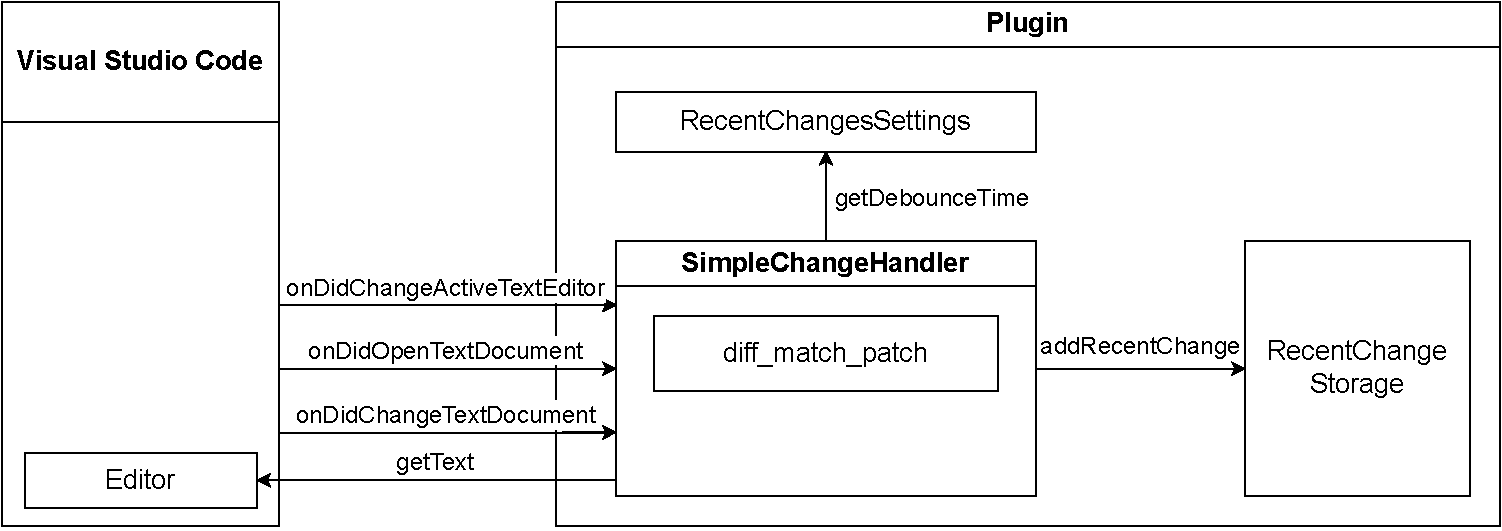
\includegraphics[width=.95\textwidth]{diagram_VSCodeDesign-Detail_Handler}
%     \caption{Detaillierte Darstellung des \emph{SimpleChangeHandler}.}
%     \label{fig:diagram_VSCodeDesign-Detail_Handler}
% \end{figure}
% \begin{figure}
%     \centering
%     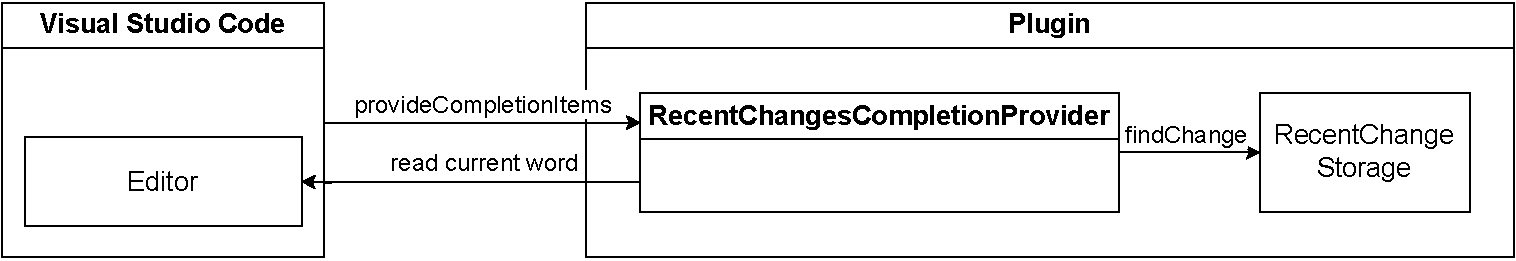
\includegraphics[width=.95\textwidth]{diagram_VSCodeDesign-Detail_Provider}
%     \caption{Detaillierte Darstellung des \emph{RecentChangesCompletionProvider}.}
%     \label{fig:diagram_VSCodeDesign-Detail_Provider}
% \end{figure}   
% \begin{figure}
%     \centering
%     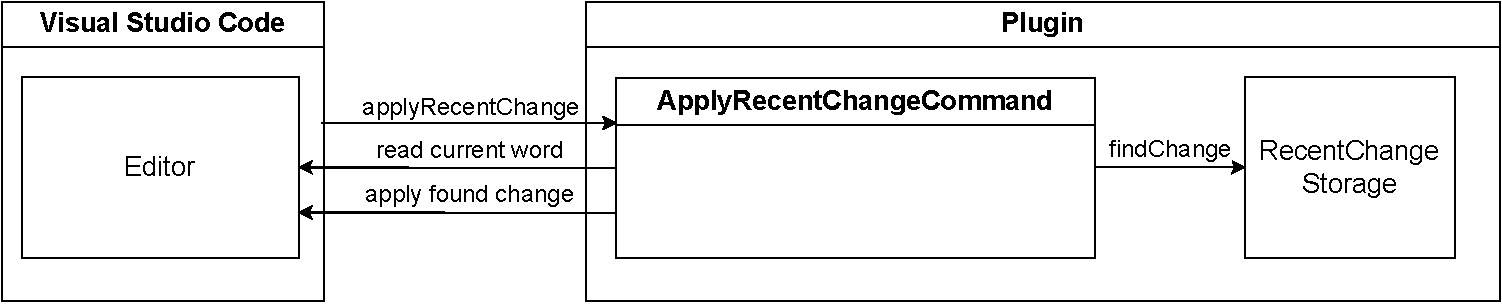
\includegraphics[width=.95\textwidth]{diagram_VSCodeDesign-Detail_Command}
%     \caption{Detaillierte Darstellung des \emph{ApplyRecentChangeCommand}.}
%     \label{fig:diagram_VSCodeDesign-Detail_Command}
% \end{figure}   
% \begin{figure}
%     \centering
%     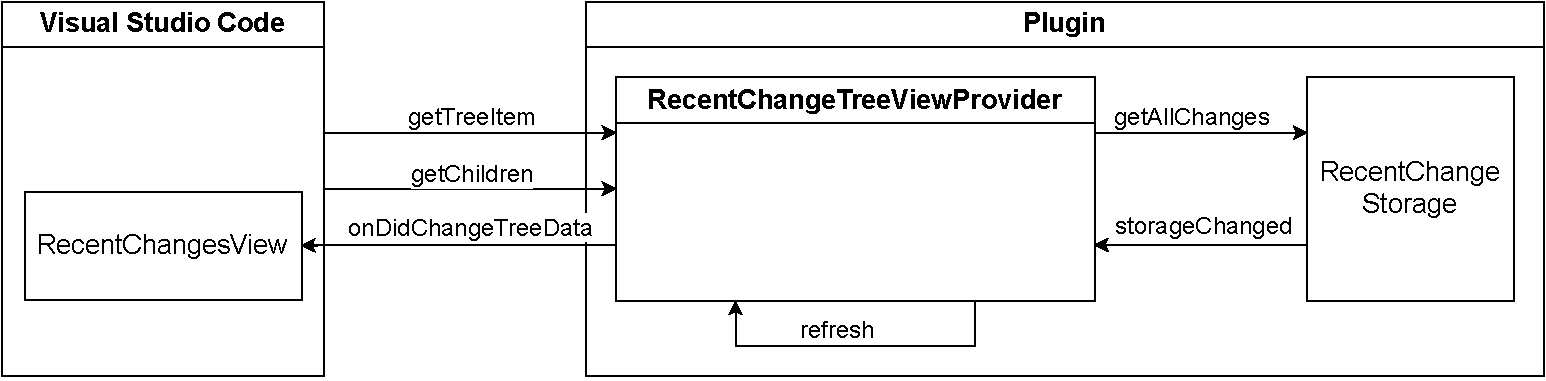
\includegraphics[width=.95\textwidth]{diagram_VSCodeDesign-Detail_TreeView}
%     \caption{Detaillierte Darstellung des \emph{RecentChangeTreeViewProvider}.}
%     \label{fig:diagram_VSCodeDesign-Detail_TreeView}
% \end{figure}   
% \begin{figure}
%     \centering
%     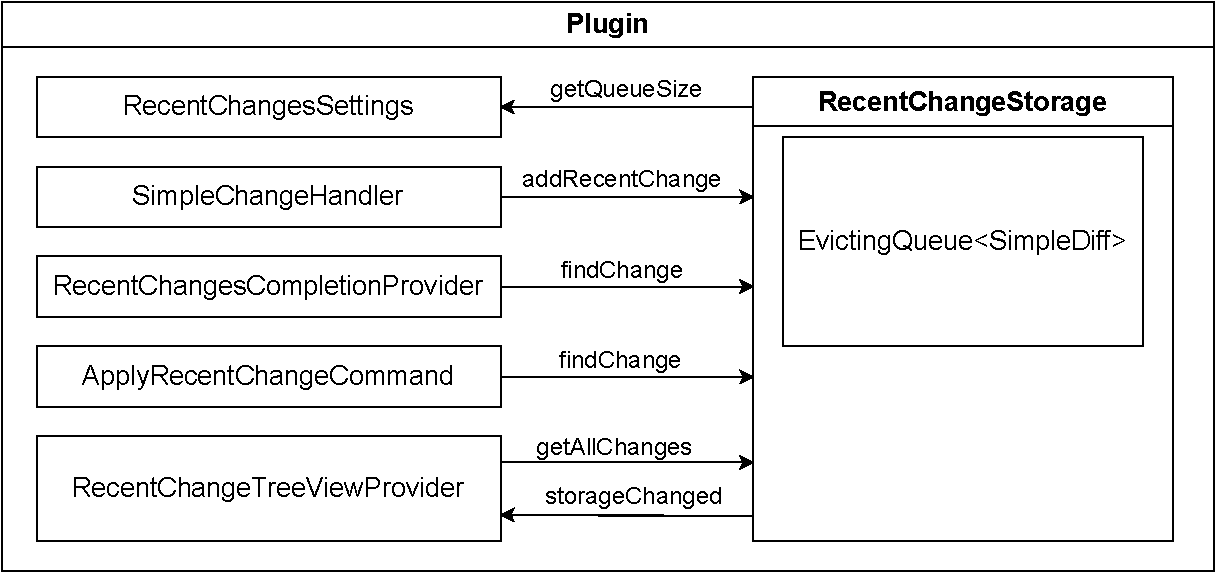
\includegraphics[width=.95\textwidth]{diagram_VSCodeDesign-Detail_Storage}
%     \caption{Detaillierte Darstellung des \emph{RecentChangeStorage}.}
%     \label{fig:diagram_VSCodeDesign-Detail_Storage}
% \end{figure}   

\section{Implementierung}
\label{sec:EntwicklungVsCode_Implementierung}

\subsection{Aufsetzen des Projektes}

% //TODO source
Um mit der Entwicklung eines VS Code Plugins zu starten, muss zuerst \emph{Node.js} % //TODO add source or link?
auf dem Gerät installiert sein. Mithilfe von Node.js können das Werkzeug
\emph{Yeoman} und ein dazugehöriger Generator mit dem Befehl
\begin{GenericCode}[numbers=none]
    npm install -g yo generator-code
\end{GenericCode}
installiert werden.
\emph{Yeoman} kann daraufhin ein Plugin-Projekt automatisch über den Befehl
\begin{GenericCode}[numbers=none]
    yo code
\end{GenericCode}
erstellen. Während dieses Erstellungsprozesses können verschiedene Einstellungen
wie der Name und die Art der Extension festgelegt werden. Generiert wird dann,
je nach vorgenommenen Einstellungen, eine Ordnerstruktur die die wichtigsten
Elemente eines Plugins beinhaltet. So wird mit den Standardeinstellungen
ein Projekt angelegt, welches bereits ein Extension Manifest, eine Datei 
\emph{extension.ts} mit dem Aktivierungs-Code und einige leere Testfälle enthält.

\begin{figure}
    \centering
    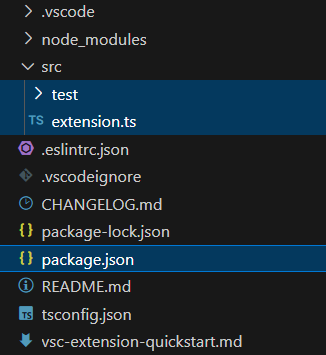
\includegraphics[width=.35\textwidth]{vscode_generated_structure}
    \caption{Durch \emph{Yeoman} generierte Ordnerstruktur.}
    \label{fig:vscode_generated_structure}
\end{figure}   

\subsection{Entwicklung}

\section{Tests}
\label{sec:EntwicklungVsCode_Tests}

\section{Publishing}
\label{sec:EntwicklungVsCode_Publishing}

% //TODO source
Das Veröffentlichen einer VS Code Extension funktioniert über das 
\emph{vsce} Komandozeilenwerkzeug. Dieses kann mithilfe des Befehls
\begin{GenericCode}[numbers=none]
    npm install -g @vscode/vsce
\end{GenericCode}
installiert werden. Das fertige Plugin kann daraufhin mit 
\begin{GenericCode}[numbers=none]
    vsce package
\end{GenericCode}
verpackt und mit 
\begin{GenericCode}[numbers=none]
    vsce publish
\end{GenericCode}
in den VS Code Marketplace hochgeladen werden.

Beim Hochladen ist zu beachten, dass ein \emph{personal access token}
und ein \emph{publisher} Name benötigt werden.
Um den Token zu erhalten, muss man zuerst in Azure DevOps eine neue Organisation
anlegen (sofern man nicht bereits Teil einer Organisation ist). In den 
Benutzereinstellungen kann ein neuer Token erstellt werden. Dabei müssen auch die 
Berechtigungen für den Token festgelegt werden. Bei dem Abschnitt für 
\emph{Marketplace} muss hier die Berechtigung \emph{Manage} gesetzt sein.
Ein Publisher kann erstellt werden indem man sich im Marketplace anmeldet
und die Seite \url{https://marketplace.visualstudio.com/manage} aufruft.
Hier gibt es einen Dialog zum Erstellen eines neuen Publishers. Dieser
Publisher benötigt mindestens eine eindeutige ID und einen eindeutigen
Namen, welche später im Marketplace angezeigt werden. Der Publisher Name
muss weiters noch in der Datei \emph{package.json} eingetragen werden.

Das Verwalten von bereits hochgeladenen Extensions kann entweder
über das Werkzeug \emph{vsce} oder über die grafische Benutzeroberfläche
im Marketplace erledigt werden.

\section{CI/CD}
\label{sec:EntwicklungVsCode_CICD}